\section{PCB}

Projekt płytki PCB został wykonany w programie \textit{Altium Designer 6.1} na licencji AGH udostępnionej przez Promotora. Postępy były archiwizowane z użyciem systemu kontroli wersji \textit{git}. Repozytorium z projektem: \url{https://gitlab.com/Hoplophile/tactical_headphones.git}.

Zastosowano globalne etykiety połączeń i podział na pliki dla lepszej przejrzystości. Do wyglądu schematów wykorzystany został szablon stworzony w ramach zajęć \textit{Podstawy projektowania obwodów z wykorzystaniem oprogramowania CAD/CAM}. 

Ponieważ użyta wersja \textit{Altiuma} nie posiada jeszcze opcji projektu wielolayoutowego, konieczne było stworzenie dwóch podprojektów. Zostały do nich dodane odpowiednie pliki z głównego projektu. Strukturę plików przedstawiono na \ref{pic:struktura}.

\begin{figure}[H]
	\centering
	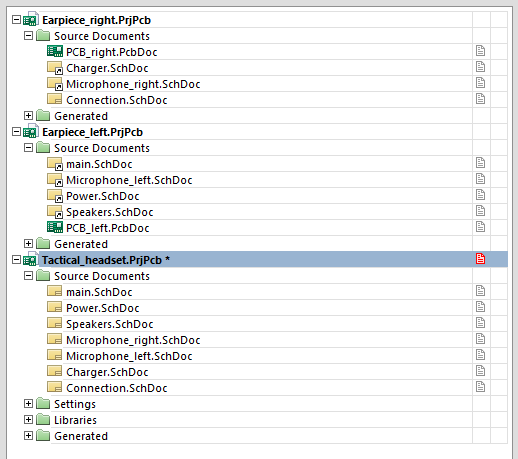
\includegraphics[scale=0.6]{zdjecia/PCB/struktura.png}
	\caption{\label{pic:struktura} Struktura plików w projektach PCB}
\end{figure}

Poniżej opisano poszczególne schematy oraz layouty składające się na projekt słuchawek.




\subsection{Main}

Plik main.sch zawiera ogólne elementy schematu, czyli: mikrokontroler, przyciski użytkownika oraz konektory do programowania, komunikacji między lewą i prawą słuchawką, mikrofonu komunikacyjnego i komunikacji radiowej.

Przewidziano 3 przyciski dla użytkownika (plus/góra, minus/dół, główny). Zostały podłączone do portów GPIO mikrokontrolera oraz do zasilania przez rezystory pull-up o wartościach $4,7k\Omega$. Wciśnięcie przycisku jest równoważne ze zwarciem danego portu do masy.

Podobnie pin \textbf{NRST} jest podłączony do zasilania przez rezystor pull-up. W pierwszych wersjach schematu był tam również podłączony przycisk TACT, jednak usunięto go, aby zaoszczędzić miejsce. Reset jest możliwy poprzez zwarcie pinu resetu na konektorze \textbf{SWD}.

Złącze do programowania jest zaprojektowane tak, aby można było flashować i debugować mikrokontroler przez złącze ST-LINK obecne na przykład na platformie Nucleo, na której wykonywany był prototyp. 

Konektor do komunikacji radiowej ma 3 piny. Pierwszy jest połączeniem do masy. Drugi przekazuje sygnał z radiotelefonu do przetwornika analogowo-cyfrowego mikrokontrolera. Trzeci jest pinem wyjściowym mikrofonu komunikacyjnego, przy którym zastosowano równolegle rezystor, ograniczający prąd zasilania mikrofonu oraz szeregowo kondensator blokujący napięcie stałe.

Do pinu $V_{REF}$ mikrokontrolera dodano dodatkowo dwa kondensatory: \textbf{C1} i \textbf{C4}. Zastosowano je później, po pierwszych próbach odczytu sygnału z mikrofonu przez wbudowany ADC, ponieważ okazało się, że jest on obarczony dużym szumem.

\begin{figure}[H]
	\centering
	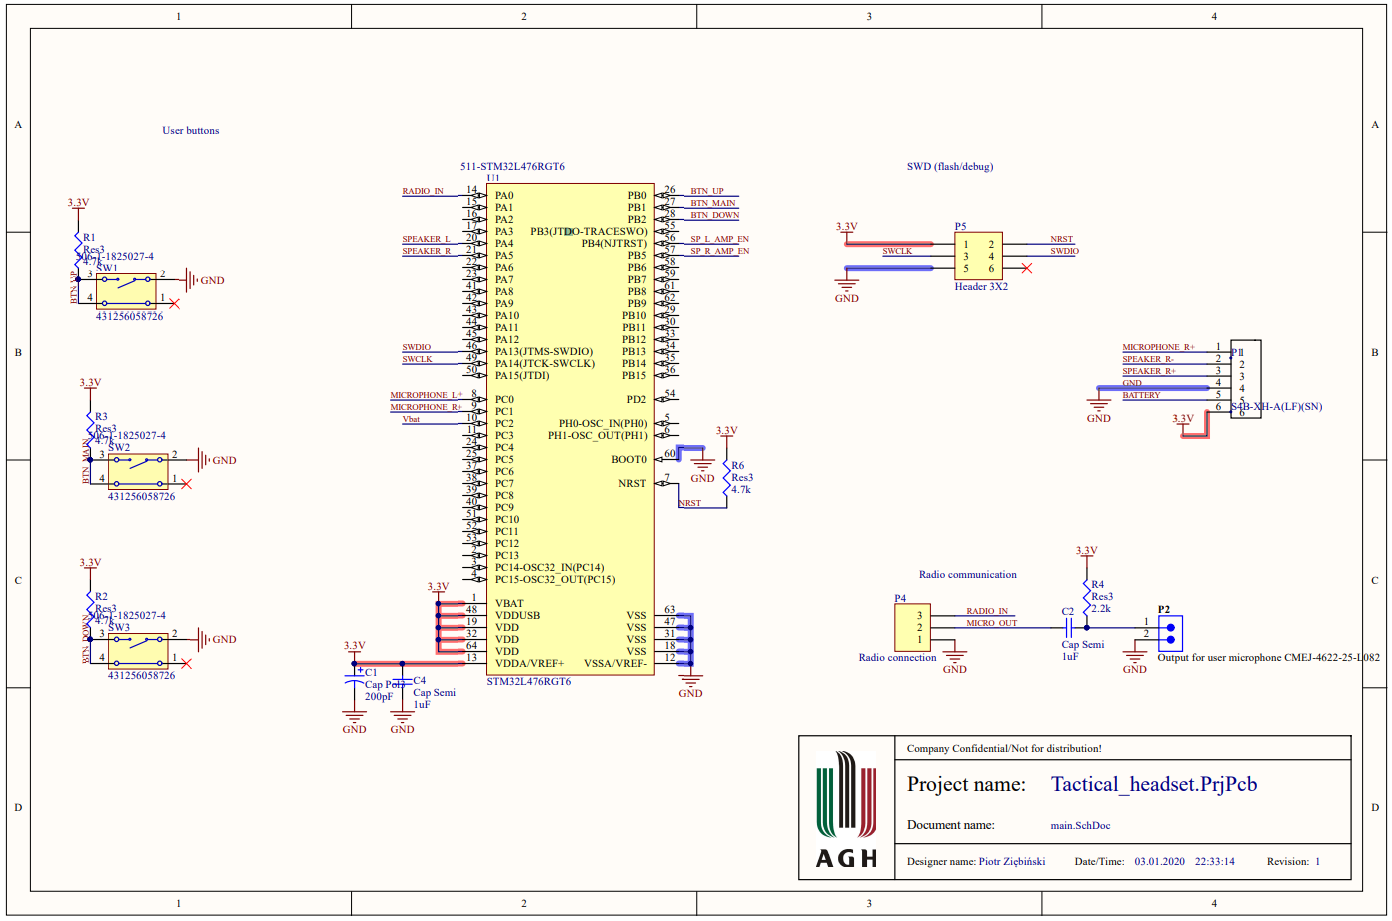
\includegraphics[scale=0.4]{zdjecia/PCB/main.png}
	\caption{\label{main} Schemat \textit{main}}
\end{figure}


\subsection{Power}

Początkowo ten plik zawierał stabilizator napięcia oraz układ ładowania do akumulatora. Na potrzeby podziału układu na dwie osobne płytki PCB, układ ładowania został przeniesiony na osobny schemat. Na głównej, lewej, płytce został stabilizator \textbf{JAKI STABILIZATOR} ustawiony na $3.3V$. Według specyfikacji jest w stanie dać \textbf{PRĄD}. Zostały dodane kondensatory filtrujące oraz cewka na wyjściu, tworzące filtr dolnoprzepustowy LC o częstotliwości granicznej \textbf{CZESTOT. NA WYJŚCIU REG}. 

Miedzy portem wejściowym baterii a masą został utworzony dzielnik napięcia z rezystorami $220k \Omega $. Było to konieczne do pomiaru poziomu naładowania baterii, ponieważ jej napięcie maksymalne wynosi $4,2V$ co wykracza poza zakres przetwornika mikrokontrolera, którego $V_{ref}$ wynosi $3,3V$. Napięcie jest dzielone przez 2, więc maksymalnie wynosi $2,1V$ i mieści się w zakresie ADC, a odczytana wartość jest mnożona dwukrotnie przez program, aby otrzymać rzeczywistą wartość. Dzięki zastosowaniu rezystorów o dużej wartości, prąd przepływający przez dzielnik przy pełnym naładowaniu baterii wynosi tylko $9,6\mu A$.

\begin{figure}[H]
	\centering
	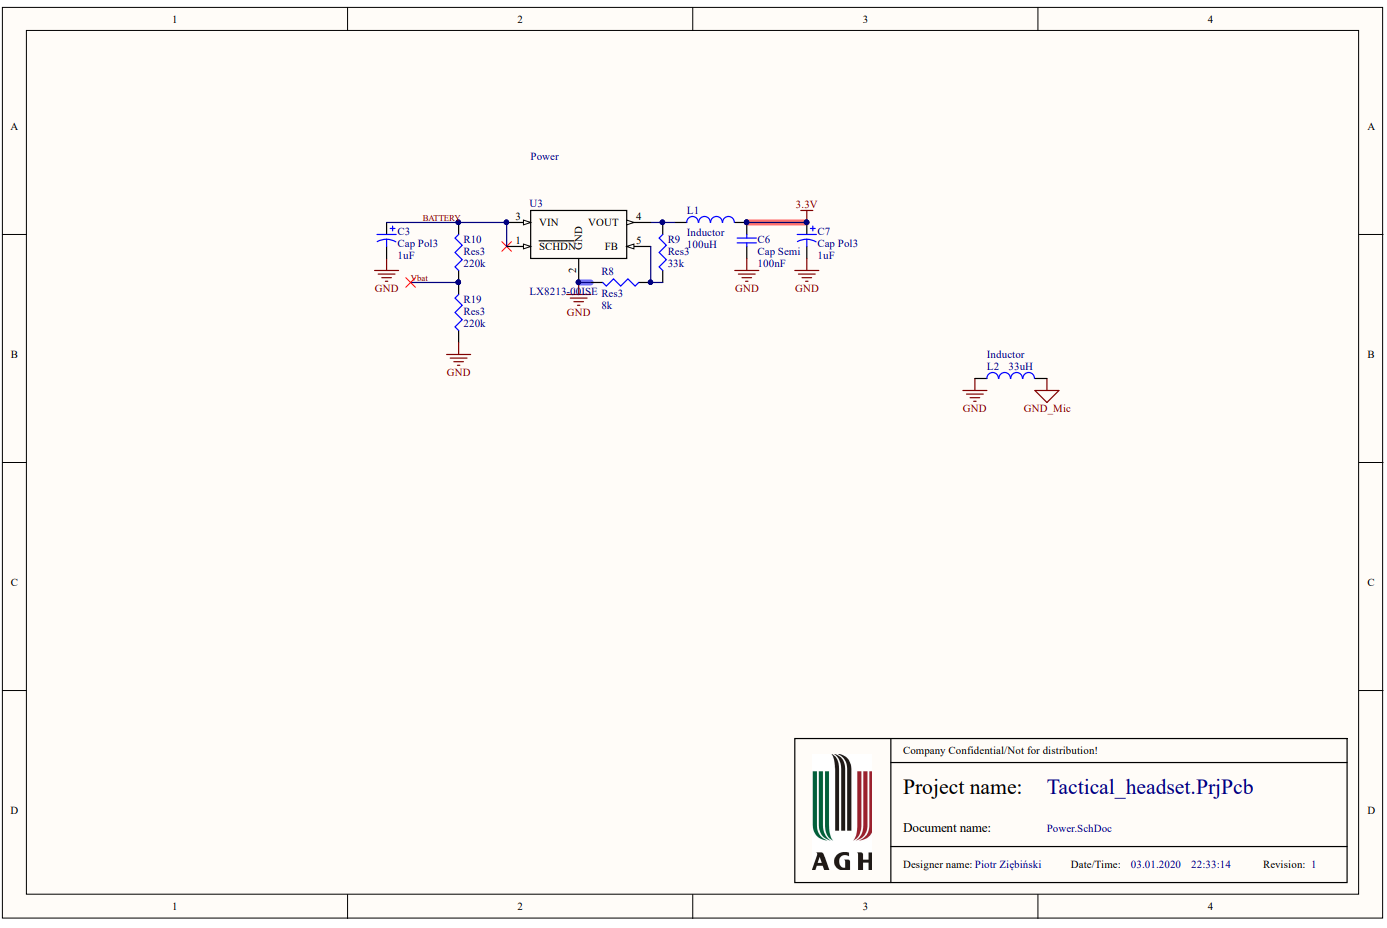
\includegraphics[scale=0.4]{zdjecia/PCB/power.png}
	\caption{\label{power} Schemat \textit{Power}}
\end{figure}


\subsection{Charger}

Układ ładujący do akumulatora został przeniesiony na osobny schemat, kiedy zdecydowano o jego umieszczeniu na drugiej płytce. Wejściem jest złącze żeńskie micro USB B, przez które dostarczane jest napięcie $5V$, natomiast wyjście jest bezpośrednio połączone z portem akumulatora. Wykorzystano również możliwość wskazywania statusu ładowania, dodając diodę LED według specyfikacji. Rezystor \textbf{R16} służy do ustawiania prądu ładowania, wybrana wartość jest równoważna z $450mA$, co jest bliskie maksymalnemu prądowi ładowania wybranego akumulatora, wynoszącemu \textbf{PRĄD ŁADOWANIA}. 

Zgodnie z zalecaną aplikacją w nocie katalogowej, dodano kondensatory na wejściu i wyjściu układu.

\begin{figure}[H]
	\centering
	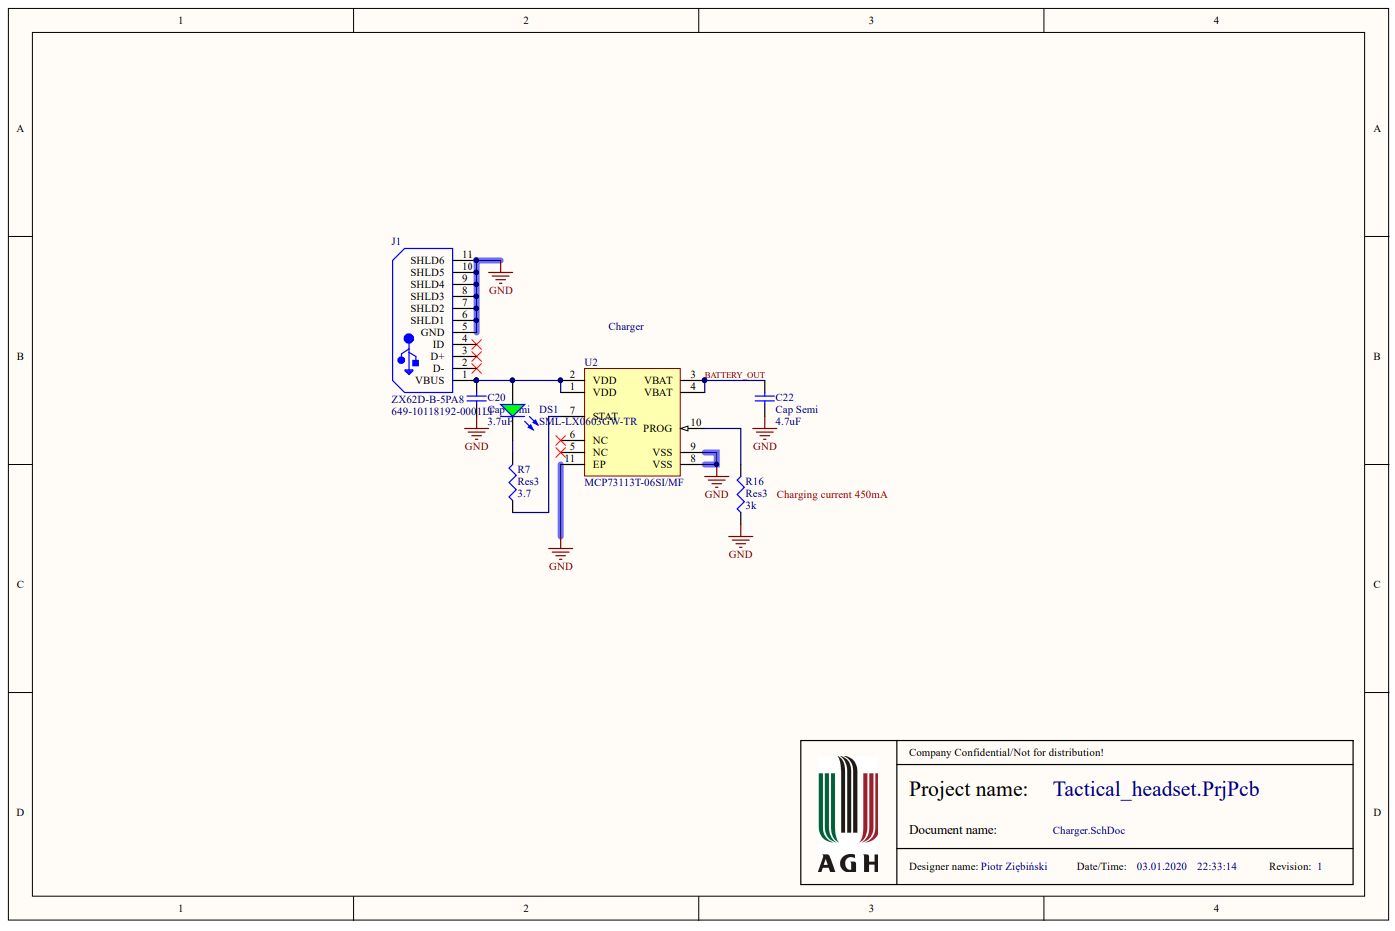
\includegraphics[scale=0.4]{zdjecia/PCB/charger.png}
	\caption{\label{charger} Schemat \textit{Charger}}
\end{figure}


\subsection{Microphone\_left i Microphone\_right}

Oba pliki zawierają bliźniacze schematy z symbolami mikrofonów \textit{SPW2430}. Oprócz nich wstawione zostały kondensatory filtrujące na zasilaniu oraz filtry dolnoprzepustowe RC na wyjściach. Podobnie jak w poprzednim przypadku - pierwotnie jeden schemat został później podzielony na dwa, ponieważ drugi mikrofon znajduje się na drugiej płytce PCB i musi być zamontowany powierzchniowo.

W projekcie zastosowano dwie rozdzielne masy. Na potrzeby filtracji szumów rozważane były różne konfiguracje i ostatecznie zdecydowano o utworzeniu osobnej masy dla mikrofonów, połączonej na obu płytkach indukcyjnością z głównym GND.

\pagebreak
\begin{figure}[H]
	\centering
	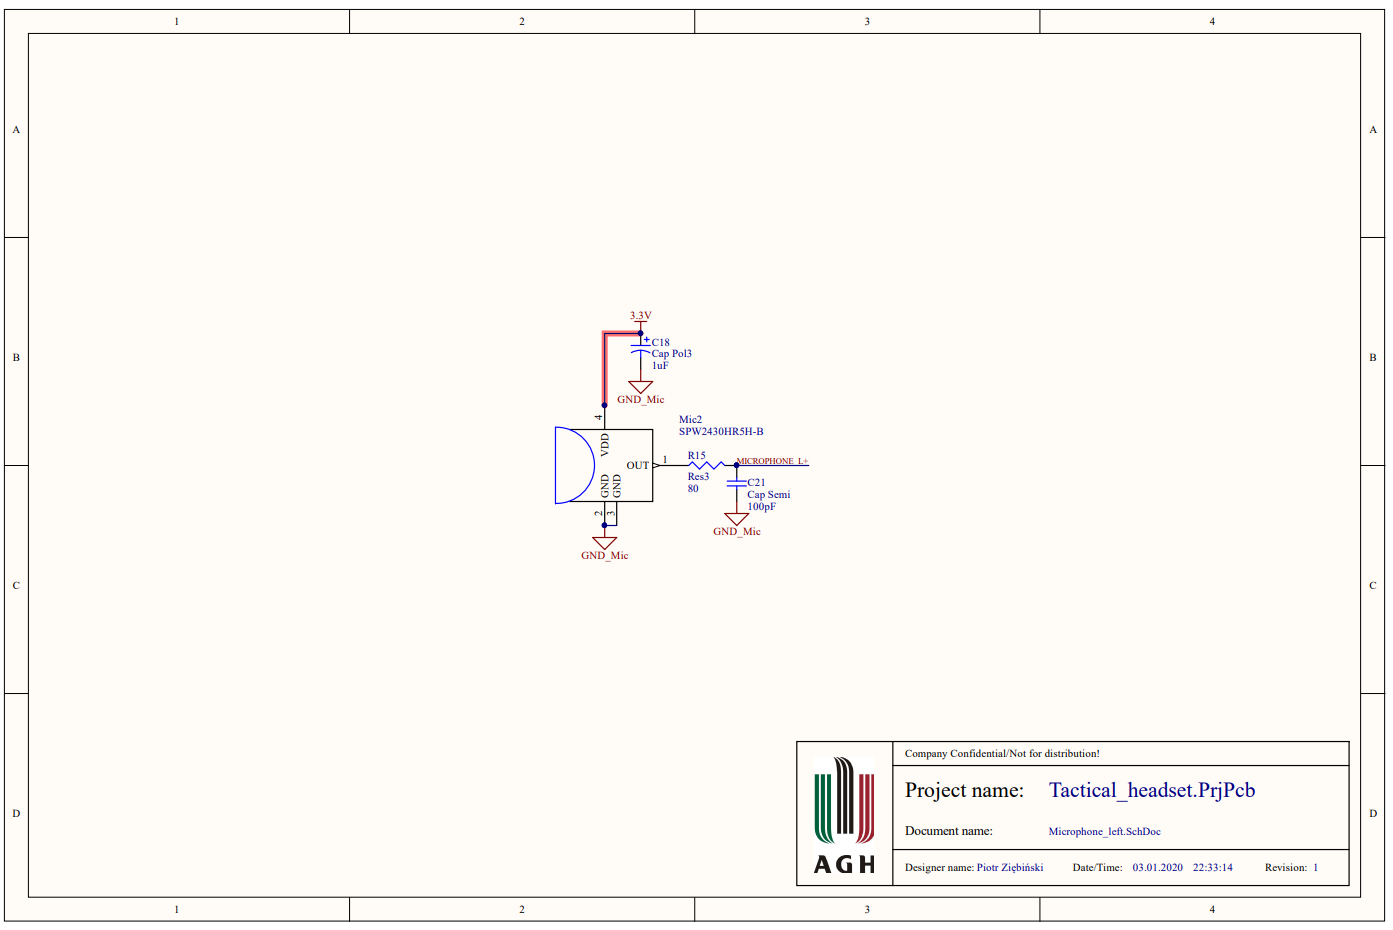
\includegraphics[scale=0.4]{zdjecia/PCB/mic_left.png}
	\caption{\label{mic_left} Schemat \textit{Microphone\_left}}
\end{figure}

\begin{figure}[H]
	\centering
	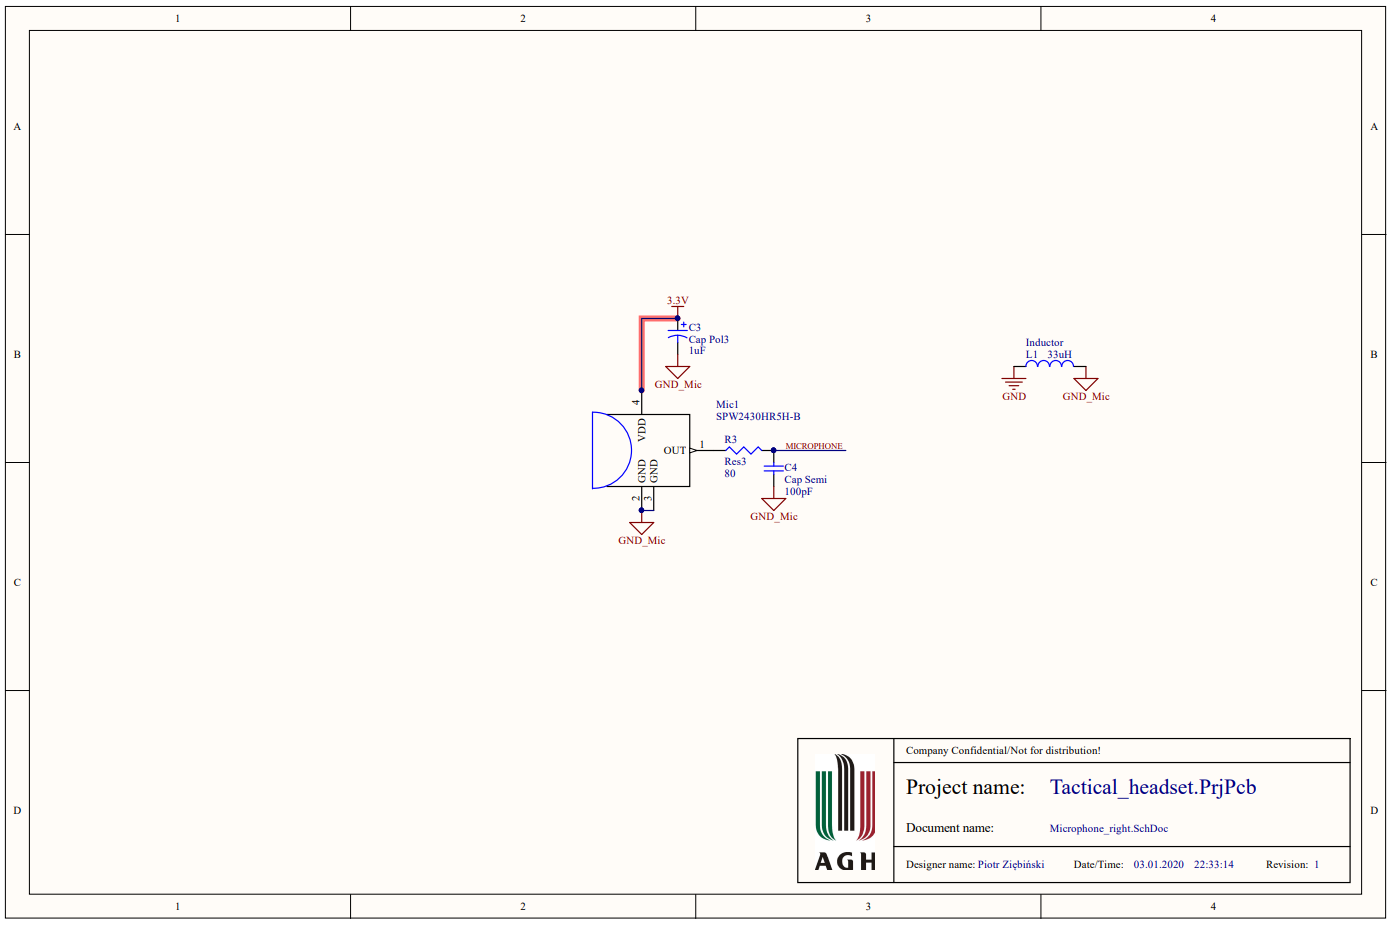
\includegraphics[scale=0.4]{zdjecia/PCB/mic_right.png}
	\caption{\label{mic_right} Schemat \textit{Microphone\_right}}
\end{figure}


\subsection{Speakers}

W przypadku głośników schemat jest wspólny, ponieważ oba wzmacniacze zostały umieszczone na głównym PCB.

Na wyjściach zastosowano filtry LC z częstotliwością graniczną $27khz$ sugerowane w specyfikacji, aby obniżyć szumy EMI. Zasilania również zostały odfiltrowane kondensatorami \textbf{C10} oraz \textbf{C15}.

Na wejściach różnicowych stworzono filtry górnoprzepustowe na $100hz$.

Piny \textbf{SHUTDOWN} zostały podłączone do mikrokontrolera w celu wyłączania wzmacniaczy w trybie uśpienia systemu. Pobierają wtedy maksymalnie $2\mu A$. 

\begin{figure}[H]
	\centering
	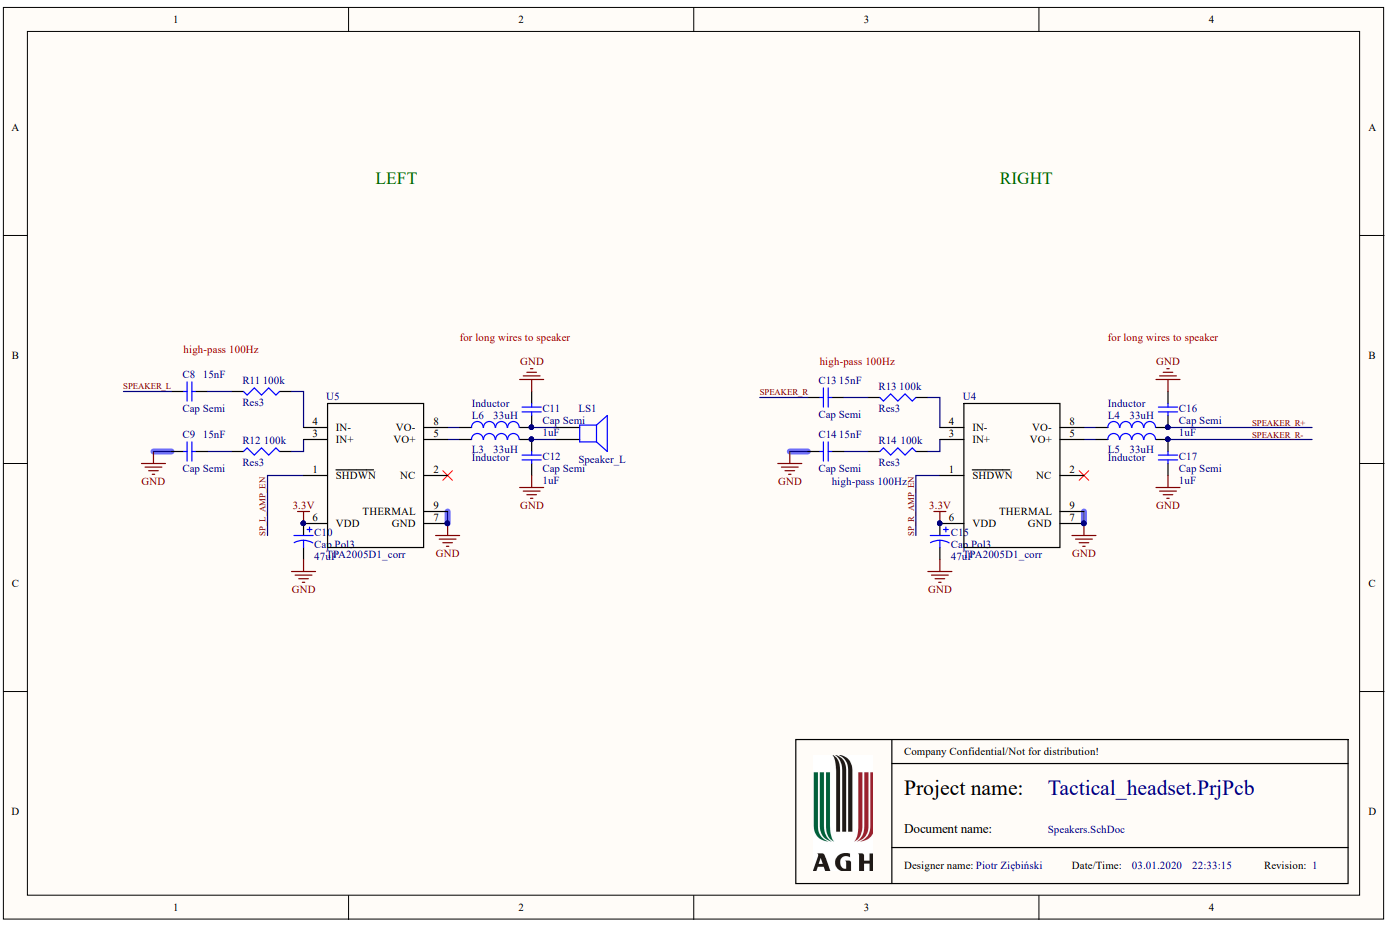
\includegraphics[scale=0.4]{zdjecia/PCB/speakers.png}
	\caption{\label{speakers} Schemat \textit{Speakers}}
\end{figure}


\subsection{Connection}

Schemat stworzony na potrzeby drugiej płytki. Znajdują się na nim: konektor komunikacyjny do głównego PCB, wyjścia do głośnika oraz baterii.

Komunikacja między płytkami odbywa się 6 przewodami: masa, zasilanie $3,3V$, napięcie baterii, dwa sygnały do głośnika i sygnał mikrofonu.

\begin{figure}[H]
	\centering
	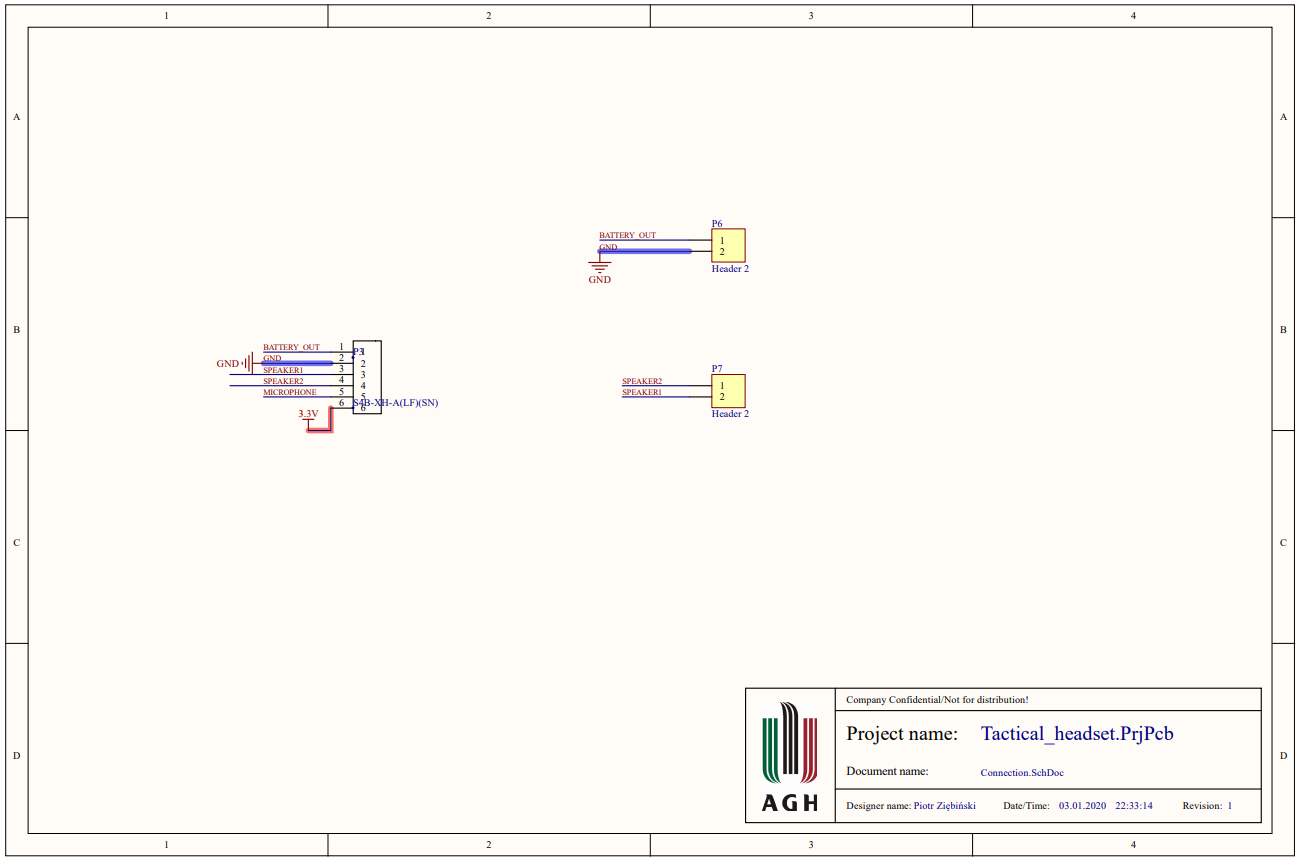
\includegraphics[scale=0.4]{zdjecia/PCB/connection.png}
	\caption{\label{connection} Schemat \textit{Connection}}
\end{figure}


\subsection{PCB\_left}

Jest to główna płytka, na której znajduje się mikrokontroler odpowiedzialny za obliczenia i przetwarzanie sygnałów. Oprócz tego umieszczono na niej przede wszystkim: przyciski, konektor do programowania, do podłączenia radiotelefonu i mikrofonu komunikacyjnego, dwa otwory montażowe wzmacniacze do głośników oraz mikrofon. Ma ona kształt ośmiokąta foremnego o całkowitej szerokości i wysokości $40mm$. Zastosowanie niewielkich wymiarów pozwoliło na łatwe umieszczenie płytki w obudowie i pozostawienie miejsca na materiał wyciszający.

Prawie wszystkie elementy, oprócz mikrofonu i filtrującego jego zasilanie kondensatora, zostały umieszczone na górnej warstwie. Te dwa elementy znajdują się na dole, ponieważ port mikrofonu musiał być skierowany na zewnątrz obudowy i być maksymalnie blisko niej. Do rezystorów zastosowano obudowy 0603, a do kondensatorów i cewek 1206. Utworzone zostały masy \textbf{GND} oraz \textbf{GND\_Mic} na dolnej i górnej warstwie. Związano z nimi także siatkę przelotek łączących obie warstwy ze sobą. Płytka posiada dwa otwory montażowe o średnicach $3,2mm$.

Do mikrofonu komunikacyjnego i połączenia między płytkami zastosowano konektory \textit{JST-XH}. Wyjście głośnika i piny do radiotelefonu przewidziano jako otwory, do których zostaną przylutowane odpowiednie przewody. Natomiast konektor \textbf{SWD} ma służyć jako punkty stykowe do kabla programatora.


\begin{figure}[H]
	\centering
	\begin{subfigure}{.45\textwidth}
		\centering
		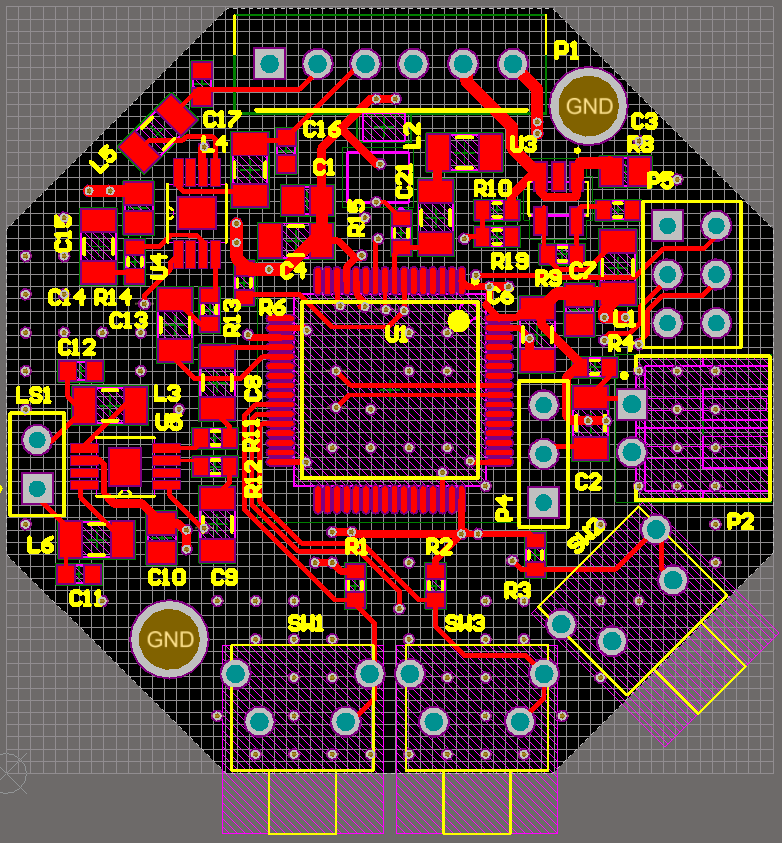
\includegraphics[height=6.5cm]{zdjecia/PCB/PCB_left_top.png}
		\subcaption{Góra}
	\end{subfigure}
	\begin{subfigure}{.45\textwidth}
		\centering
		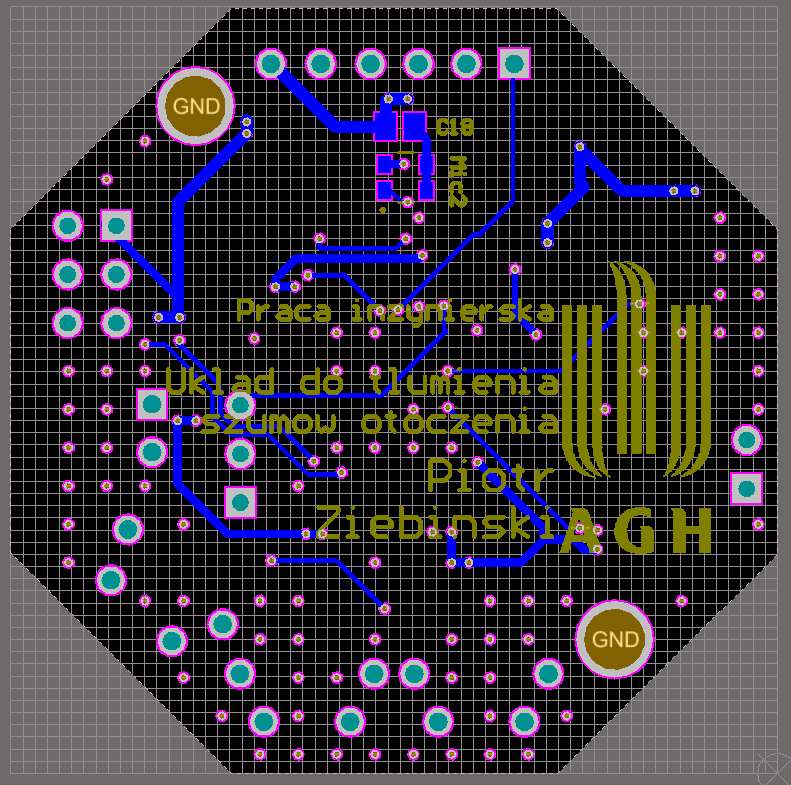
\includegraphics[height=6.5cm]{zdjecia/PCB/PCB_left_bottom.png}
		\subcaption{Dół}
	\end{subfigure}
	\caption{\label{PCB_left} Layout lewej płytki PCB}
\end{figure}

\begin{figure}[H]
	\centering
	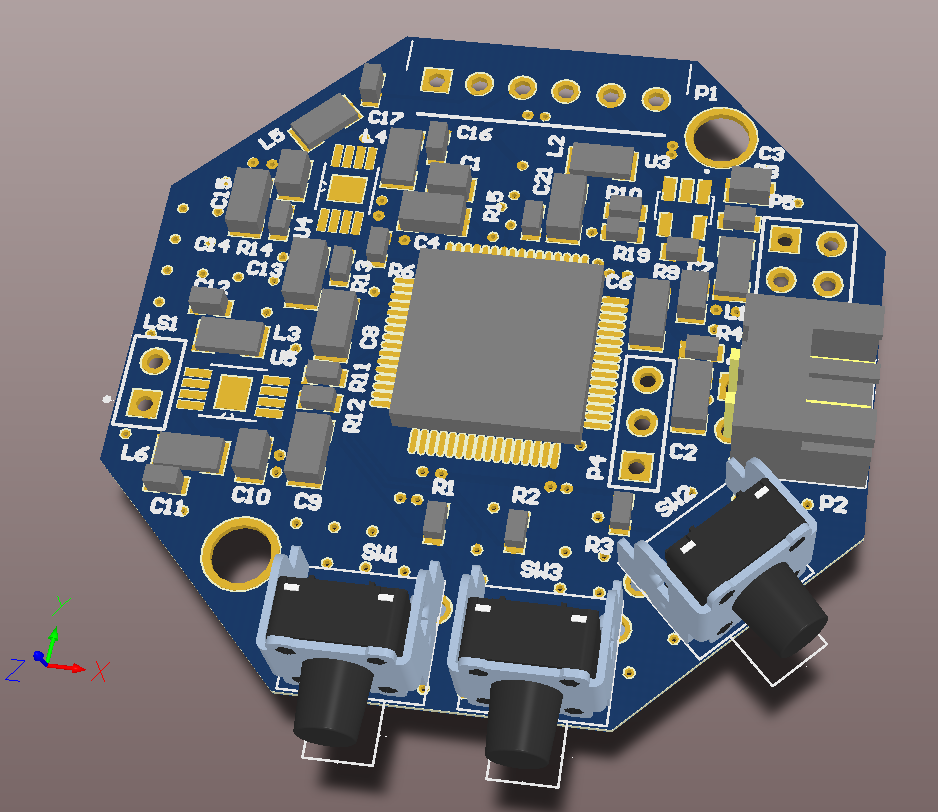
\includegraphics[scale=0.4]{zdjecia/PCB/PCB_left_3D.png}
	\caption{\label{PCB_left_3D} Wygląd płytki z góry w trybie podglądu 3D}
\end{figure}


\subsection{PCB\_right}

Płytka prawa ma znacznie bardziej ograniczoną funkcjonalność. Z tego powodu jej kształt został ograniczony do prostokąta o wymiarach $15x30mm$. 

Podobnie jak w lewej, tylko mikrofon i kondensator na jego zasilaniu, znajdują się na dolnej warstwie. Płytka zawiera oprócz tego konektor do połączenia do drugiej płytki, wyjścia głośnika i baterii oraz układ ładujący z konektorem mikro USB typu B. Również zastosowano tutaj otwory montażowe oraz po dwie masy na warstwę i dla każdej sieć przelotek.

\begin{figure}[H]
	\centering
	\begin{subfigure}{.45\textwidth}
		\centering
		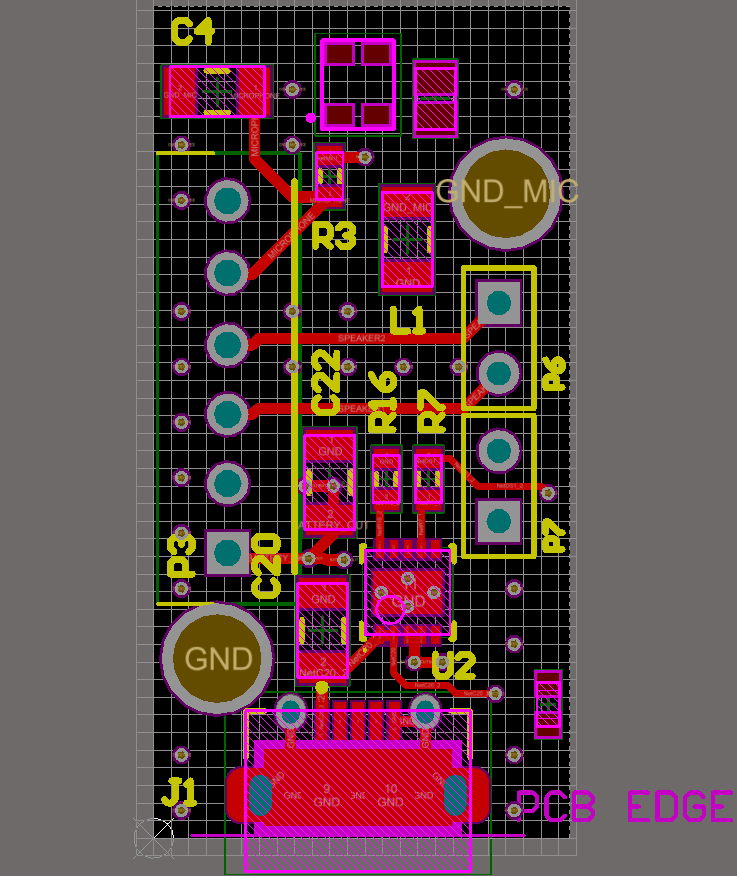
\includegraphics[height=6.5cm]{zdjecia/PCB/PCB_right_top.png}
		\subcaption{Góra}
	\end{subfigure}
	\begin{subfigure}{.45\textwidth}
		\centering
		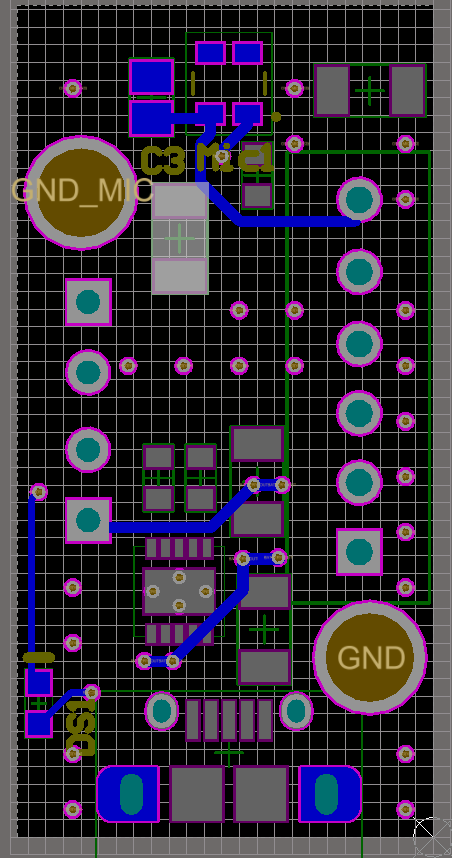
\includegraphics[height=6.5cm]{zdjecia/PCB/PCB_right_bottom.png}
		\subcaption{Dół}
	\end{subfigure}
	\caption{\label{PCB_right} Layout prawej płytki PCB}
\end{figure}

\begin{figure}[H]
	\centering
	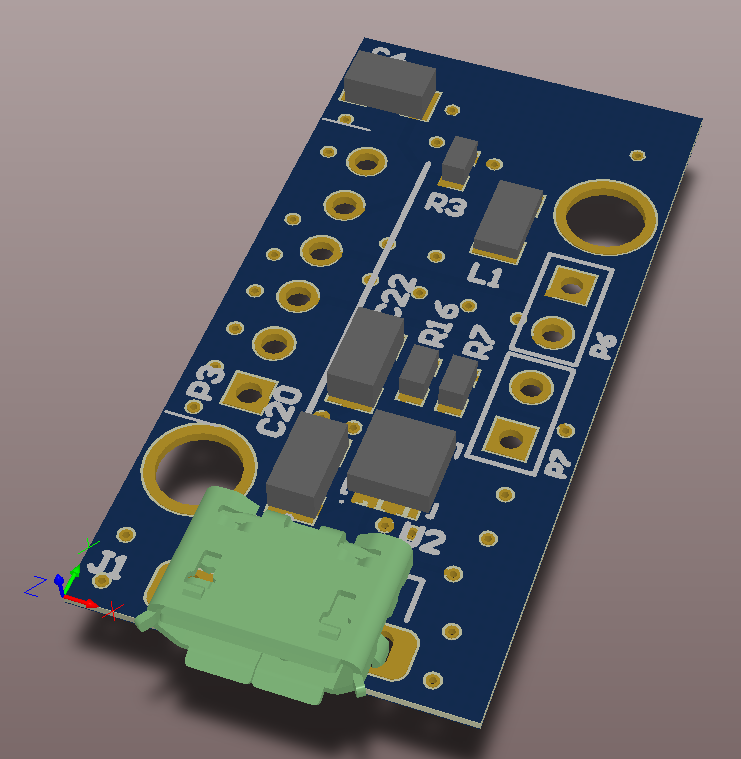
\includegraphics[scale=0.4]{zdjecia/PCB/PCB_right_3D.png}
	\caption{\label{PCB_right_3D} Wygląd prawej płytki z góry w trybie podglądu 3D}
\end{figure}
